\let\negmedspace\undefined
\let\negthickspace\undefined
\documentclass[journal]{IEEEtran}
\usepackage[a5paper, margin=10mm, onecolumn]{geometry}
\usepackage{lmodern} 
\usepackage{tfrupee} 
\setlength{\headheight}{1cm}
\setlength{\headsep}{0mm}   

\usepackage{gvv-book}
\usepackage{gvv}
\usepackage{cite}
\usepackage{amsmath,amssymb,amsfonts,amsthm}
\usepackage{algorithmic}
\usepackage{graphicx}
\usepackage{textcomp}
\usepackage{xcolor}
\usepackage{txfonts}
\usepackage{listings}
\usepackage{enumitem}
\usepackage{mathtools}
\usepackage{gensymb}
\usepackage{comment}
\usepackage[breaklinks=true]{hyperref}
\usepackage{tkz-euclide} 
\usepackage{listings}                             
\def\inputGnumericTable{}                                 
\usepackage[latin1]{inputenc}                                
\usepackage{color}                                            
\usepackage{array}                                            
\usepackage{longtable}                                       
\usepackage{calc}                                             
\usepackage{multirow}                                         
\usepackage{hhline}                                           
\usepackage{ifthen}                                           
\usepackage{lscape}
\usepackage{xparse}

\bibliographystyle{IEEEtran}

\title{2.5.25}
\author{EE25BTECH11059 - Vaishnavi Ramkrishna Anantheertha}

\begin{document}
\maketitle

\renewcommand{\thefigure}{\theenumi}
\renewcommand{\thetable}{\theenumi}

\numberwithin{equation}{enumi}
\numberwithin{figure}{enumi} 

\textbf{Question}:
Let $\mathbb{R}^3$ denote the three-dimensional space. 
Take two points $P = (1,2,3)$ and $Q = (4,2,7)$. 
Let $\text{dist}(X,Y)$ denote the distance between two points $X$ and $Y$ in $\mathbb{R}^3$. 

Let
\[
S = \{X \in \mathbb{R}^3 : (\text{dist}(X,P))^2 - (\text{dist}(X,Q))^2 = 50 \}
\]
and
\[
T = \{Y \in \mathbb{R}^3 : (\text{dist}(Y,Q))^2 - (\text{dist}(Y,P))^2 = 50 \}.
\]

Then which of the following statements are TRUE? 

\begin{enumerate}
    \item[(a)] There is a triangle whose area is $1$ and all of whose vertices are from $S$.
    \item[(b)] There are two distinct points $L$ and $M$ in $T$ such that each point on the line segment $LM$ is also in $T$.
    \item[(c)] There are infinitely many rectangles of perimeter $48$, two of whose vertices are from $S$ and the other two vertices are from $T$.
    \item[(d)] There is a square of perimeter $48$, two of whose vertices are from $S$ and the other two vertices are from $T$.
\end{enumerate}.
\\
\textbf{Solution: }\\
\begin{table}[H]    
  \centering
  \begin{tabular}{|c|c|}
\hline
\textbf{Variable} & \textbf{Value} \\
\hline
$A$ & $(0,-\frac{3}{2})$ \\
\hline
$m$ & $\frac{1}{2}$ \\
\hline
\end{tabular}
  \caption{Variables Used}
  \label{tab:1.10.25}
\end{table}

\begin{align}
                                     \vec{P}= \myvec{
                                             1
                                              \\
                                              2
                                               \\
                                               3
                                              }
\end{align}
\begin{align}
                                     \vec{Q}= \myvec{
                                             4
                                              \\
                                              2
                                               \\
                                               7
                                              }
\end{align}
\begin{align}
 \text{dist}(X,P))^2 - (\text{dist}(X,Q))^2 = 50 \\
 (\|\vec{X}-\vec{P}\|_2)^2- (\|\vec{X}-\vec{Q}\|_2)^2=50
\end{align}
\begin{align}
\vec{X^T}\vec{X}-2\vec{P^T}\vec{X}+\vec{P^T}\vec{P}-\vec{X^T}\vec{X}
+2\vec{Q^T}\vec{X}-\vec{Q^T}\vec{Q}=50\\
2(\vec{Q^T}-\vec{P^T})\vec{X}+\vec{P^T}\vec{P}-\vec{Q^T}\vec{Q}=50
\end{align}
(0.6)is the eq of plane S
\begin{align}
\text{dist}(Y,Q))^2 - (\text{dist}(Y,P))^2 = 50\\
 (\|\vec{Y}-\vec{Q}\|_2)^2- (\|\vec{Y}-\vec{P}\|_2)^2=50
\end{align}
\begin{align}
\vec{Y^T}\vec{Y}-2\vec{Q^T}\vec{Y}+\vec{Q^T}\vec{Q}-\vec{Y^T}\vec{Y}
+2\vec{P^T}\vec{Y}-\vec{P^T}\vec{P}=50\\
2(\vec{P^T}-\vec{Q^T})\vec{Y}+\vec{Q^T}\vec{Q}-\vec{P^T}\vec{P}=50
\end{align}
(0.10) is the eq of plane T\\
S And T are parallel planes\\
S is an infinite plane. In any plane one can choose three non collinear points whose triangle has unit area.Therefore a) is correct 
\\
\\
let eq of T be $\vec{n^T}\vec{X}=c$\\
let $\vec{A},\vec{B}$ be two points on T\\
\begin{align}
    \vec{n^T}\vec{A}=c\\
    \vec{n^T}\vec{B}=c
\end{align}
any point on line AB can be written as
\begin{align}
    \vec{C}=(1-k)\vec{A}+k\vec{B}\\
    \vec{n^T}[(1-k)\vec{A}+k\vec{B}]
   = \vec{n^T}\vec{A}+k[\vec{n^T}\vec{B}-\vec{n^T}\vec{A}]
   =c\\
   \vec{n^T}\vec{C}=c
\end{align}
Hence C lies on T \\
Therefore b) is correct\\
distance between S and T=$\frac{\lvert c_1 - c_2 \rvert}{|n|}
=10$\\
let $\vec{A},\vec{B}$ lie on S and $\vec{A'},\vec{B'}$
where 
\begin{align}
 \|\vec{A}-\vec{B}\|_2=\|\vec{A'}-\vec{B'}\|_2=d(say)\\
 2(d+10)=48\\
 d=14
\end{align}

There are infinitely many ways to pick two points in plane 
S that are 14 units apart (because the plane is infinite).\\
Therefore c) is correct\\
\\

The distance between the planes $S$ and $T$ is $10$. A square with perimeter $48$ has side length $12$.  
If two opposite vertices lie on $S$ and the other two on $T$, then each side of the square must connect the two planes.  
Since the vertical separation is $10$, and the side is $12$, the square can be tilted so that part of the side length is vertical ($10$ units) and the rest is horizontal: ($\sqrt{12^2 - 10^2} = \sqrt{44}$ units)


Hence d) is correct\\
Refer to Figure

\begin{figure}[H]
\begin{center}
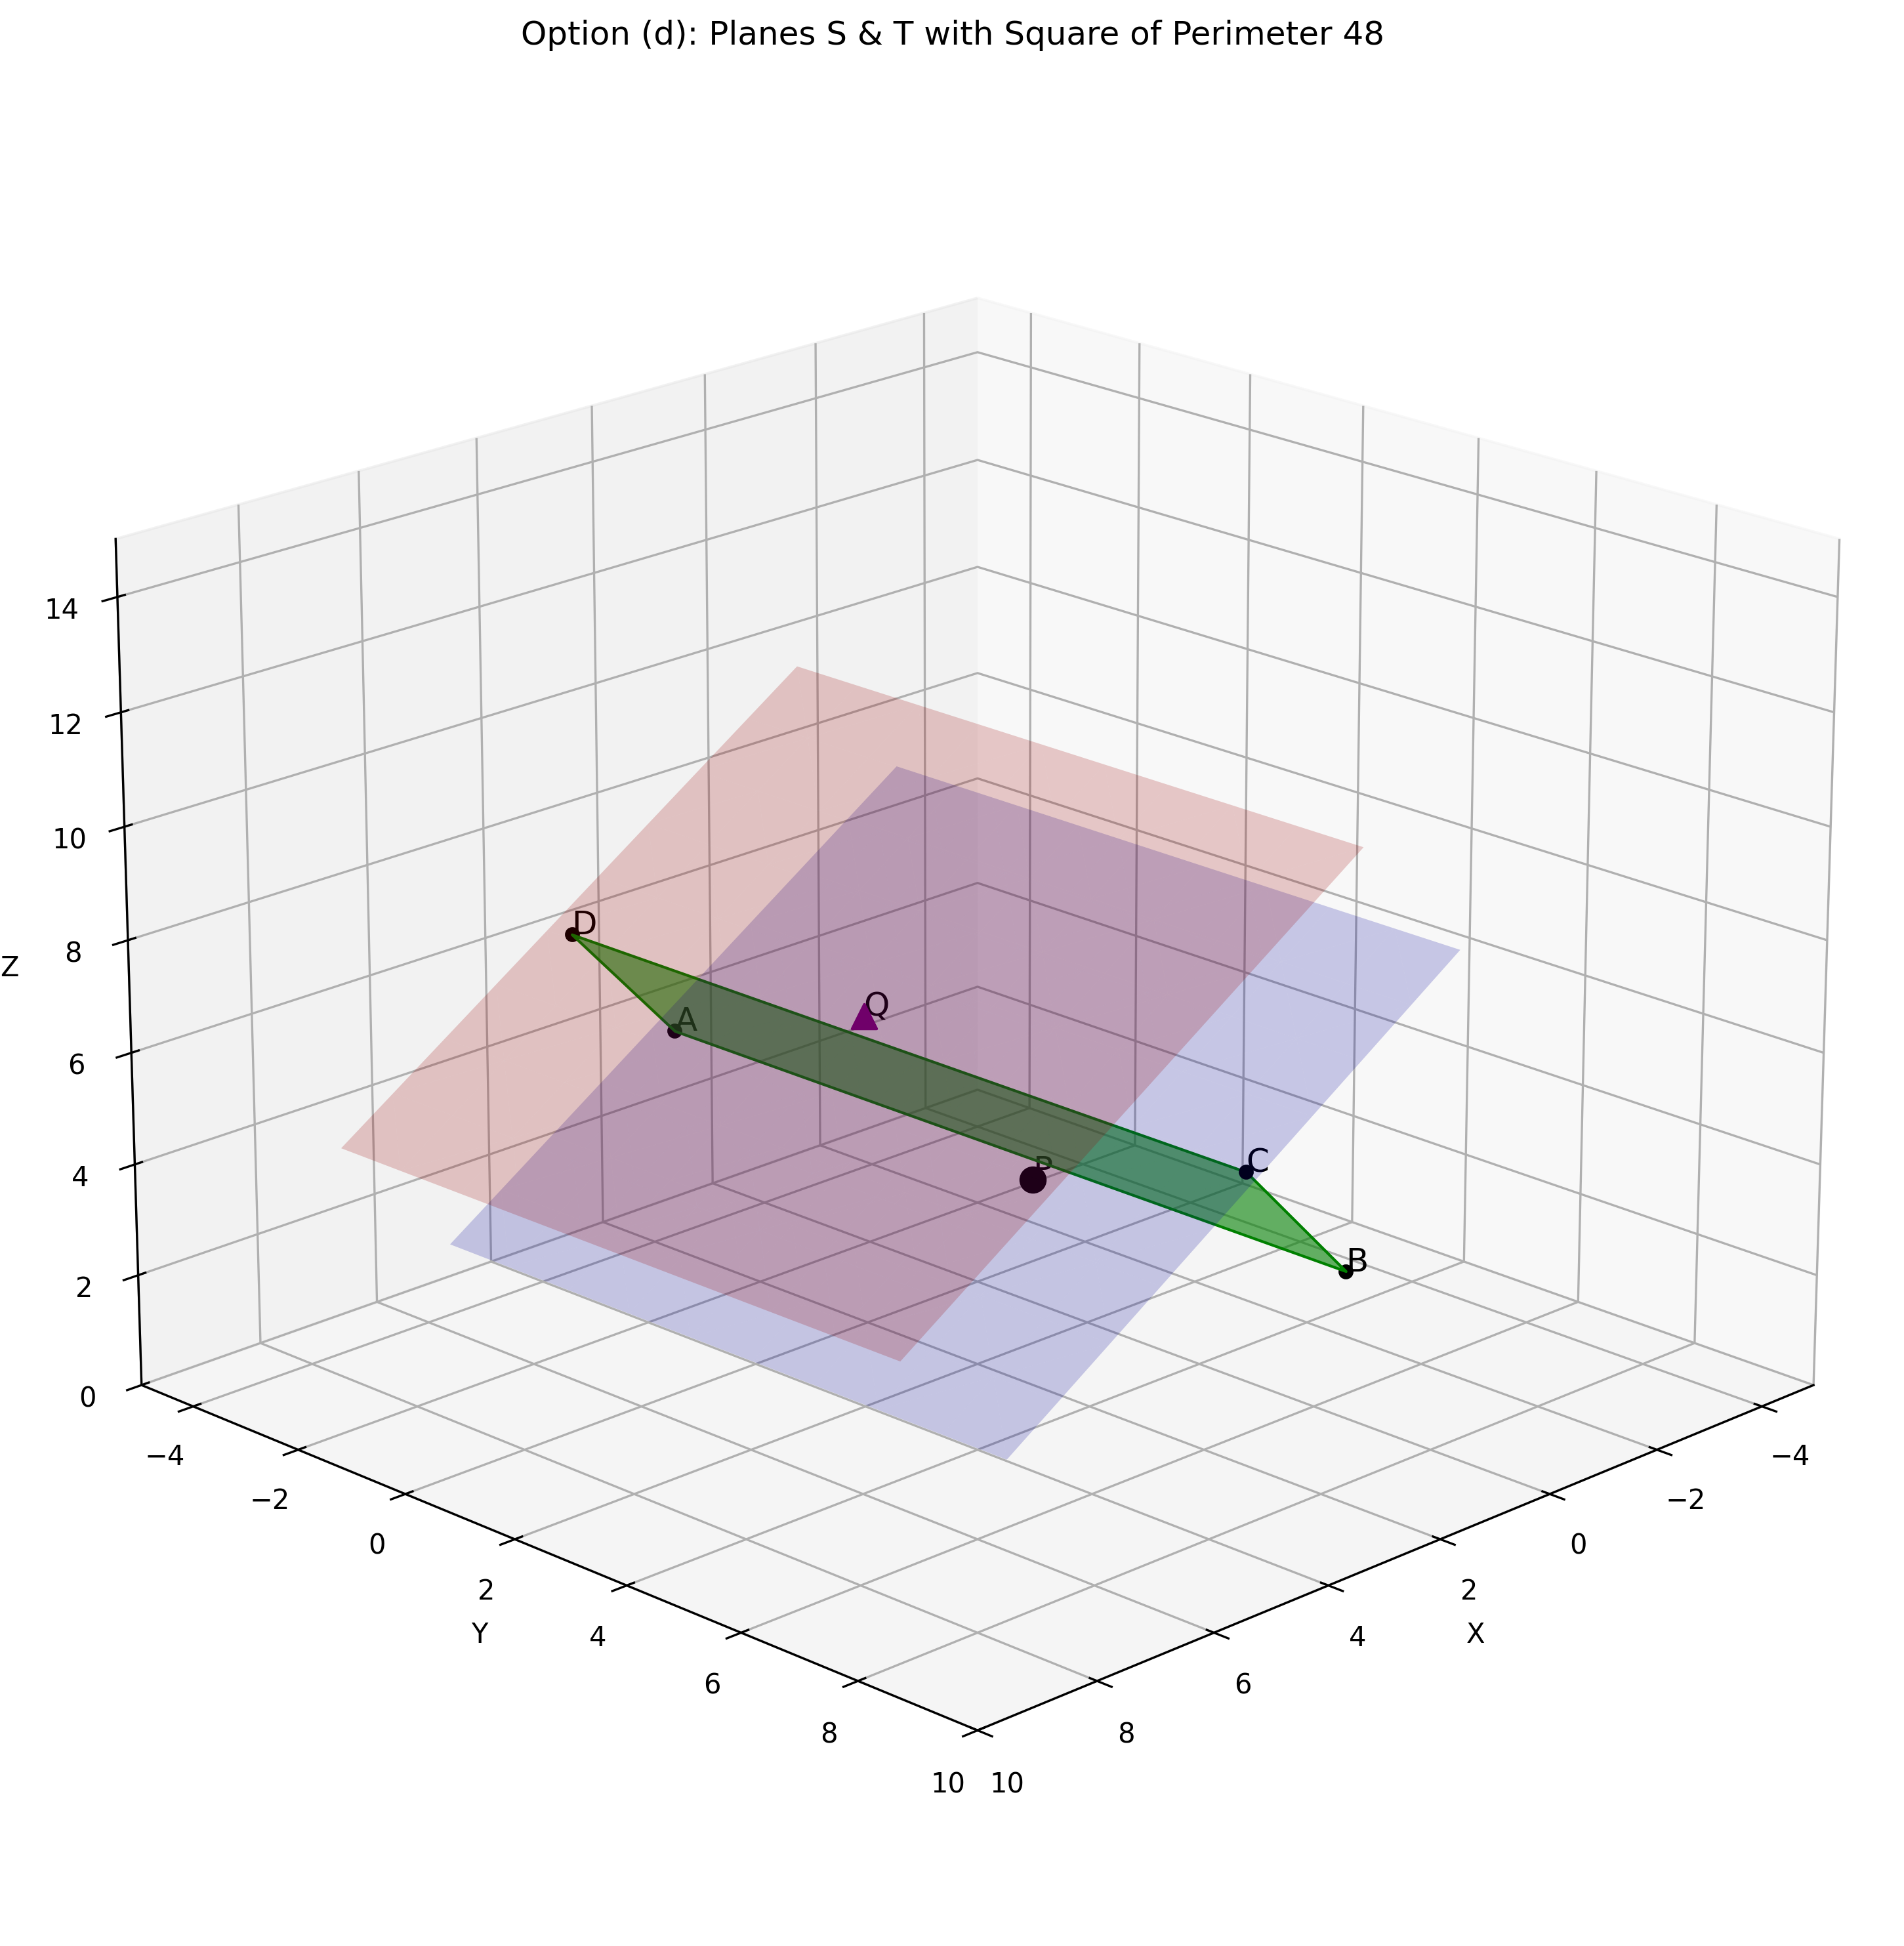
\includegraphics[width=0.6\columnwidth]{figs/graph5a.png}
\end{center}
\caption{}
\label{fig:Fig}
\end{figure}
\end{document}  